\documentclass[runningheads]{llncs}

% Paquetes necesarios
\usepackage[utf8]{inputenc}
\usepackage[spanish]{babel}
\usepackage{listings}
\usepackage{xcolor}
\usepackage{graphicx} % Necesario para figuras
\usepackage{hyperref} % Necesario para hipervínculos y referencias
\usepackage{amsmath} 
\usepackage{pdfpages}
\usepackage{float}% Necesario para el entorno align de las ecuaciones

% Configuración del estilo para listados de código
\lstset{
    basicstyle=\ttfamily\small,
    numbers=left,
    numberstyle=\tiny\color{gray},
    stepnumber=1,
    numbersep=8pt,
    backgroundcolor=\color{white},
    showspaces=false,
    showstringspaces=false,
    frame=single,
    rulecolor=\color{black!30},
    tabsize=2,
    breaklines=true,
    breakatwhitespace=true,
    captionpos=b % Leyenda debajo del código
}

\begin{document}

\title{Implementación de Estructuras Web en el Contexto de LNCS}
\author{Nicolas Sarmiento Lugones\inst{1}}
\institute{Universidad Nacional de Cuyo}

\maketitle

\begin{abstract}
Este documento presenta un ejemplo práctico de cómo incluir código fuente de lenguajes de marcado, específicamente HTML, Markdown y \LaTeX, dentro de la plantilla oficial de Springer LNCS.
\end{abstract}

\section{Introducción}
En el desarrollo de aplicaciones web y en la documentación técnica, la estructura básica se define mediante etiquetas y marcas. A continuación, se detalla la sintaxis recomendada para estos lenguajes estándar.

\section{Ejemplo Ampliado de Código HTML}
El siguiente listado muestra la estructura de una página, integrando hipervínculos, listas, tablas, figuras y formato de texto. Note el resaltado de etiquetas y atributos.

\begin{lstlisting}[language=HTML, keywordstyle=\color{blue}\bfseries, stringstyle=\color{orange}, commentstyle=\color{gray}\itshape, caption={Elementos avanzados de un documento HTML5.}, label={list:html_ejemplo}]
<!DOCTYPE html>
<html lang="es">
<head>
    <meta charset="UTF-8">
    <title>Apuntes Universitarios</title>
</head>
<body>
    <h1>Portal de <b>Ingeniería Industrial</b></h1>
    <p>Resúmenes de <i>Termodinámica</i>.</p>

    <hr>

    <a href="#materias">Ver Materias (Ancla Interna)</a><br>
    <a href="https://www.uncuyo.edu.ar/" target="_blank">Sitio UNCUYO (Externo)</a>

    <img src="diagrama.jpg" alt="Diagrama de procesos" width="300">

    <h3 id="materias">Materias cursadas:</h3>
    <ul>
        <li>Termodinámica</li>
        <li>Electrotecnia</li>
    </ul>

    <h3>Calificaciones</h3>
    <table border="1">
        <tr>
            <th>Materia</th>
            <th>Nota</th>
        </tr>
        <tr>
            <td>Termodinámica</td>
            <td>9</td>
        </tr>
    </table>
</body>
</html>
\end{lstlisting}

Para conocer más sobre estas etiquetas, se recomienda consultar la Cheatsheet de HTML \cite{mdn_html_cheatsheet}.

\section{Lenguaje de Marcas: Markdown}
Markdown permite escribir usando un formato de texto plano fácil de leer, que luego se convierte estructuralmente en HTML.

\begin{lstlisting}[language=bash, caption={Sintaxis estándar en Markdown.}, label={list:markdown}]
# Apuntes de Ingeniería
## Análisis Matemático 1

Este apunte es *estructurado* y fácil de leer.

### Contenido:
* Derivadas
* Integrales

[Ir a Notion](https://www.notion.so)
\end{lstlisting}

Referencia rápida disponible en la Cheatsheet de Markdown \cite{markdown_cheatsheet}.

\section{GitHub Flavored Markdown (Github.md)}
Esta variante añade funcionalidades nativas orientadas a la gestión operativa y de proyectos.

\begin{lstlisting}[language=bash, caption={Sintaxis de GitHub Flavored Markdown.}, label={list:gfm}]
# Tareas de Gestion (Finca)

- [x] Configurar base de datos en Notion.
- [ ] Calcular aplicacion de productos.

| Insumo | Estado |
|--------|--------|
| Abono  | OK     |
\end{lstlisting}

Referencia rápida en la Cheatsheet de GitHub Markdown \cite{github_markdown_cheatsheet}.

\section{Estructuras en \LaTeX}
\LaTeX{} es el estándar para la documentación académica de alta calidad, permitiendo una separación total entre diseño y contenido.

\begin{lstlisting}[language=TeX, caption={Sintaxis básica en \LaTeX.}, label={list:latex}]
\documentclass{article}
\begin{document}
\section{Física}
La ecuacion de la energia es $E = mc^2$.
\end{document}
\end{lstlisting}

Se puede consultar la guía rápida en la Cheatsheet de \LaTeX{} \cite{latex_cheatsheet}.

\section{Conclusión}
La incorporación de lenguajes de marcado como HTML, Markdown y \LaTeX{} significó una mejora importante en mi manera de organizar, desarrollar y presentar información técnica. Aprender a trabajar con este tipo de herramientas me permitió pasar de un uso más limitado de los procesadores de texto tradicionales a un entorno mucho más preciso, ordenado y profesional, en el que es posible distinguir claramente entre el contenido y su presentación visual. Esto no solo optimiza la redacción, sino que también facilita la estandarización y la calidad final de los documentos.

En cuanto a su proyección a futuro, considero que estas herramientas tendrán un papel fundamental en mi formación y desempeño dentro de la Ingeniería Industrial. En particular, \LaTeX{} se presenta como una opción muy valiosa para la elaboración de informes técnicos, trabajos académicos, presentaciones y también para el diseño de un currículum con formato profesional. Del mismo modo, el manejo de Markdown y HTML amplía mis posibilidades para estructurar apuntes, resúmenes y otros materiales de estudio de forma clara, adaptable y visualmente prolija, incluso con vistas a su publicación o difusión en plataformas digitales.

Por último, y tal como lo requiere la consigna, recurrí al apoyo de la Inteligencia Artificial para elaborar la tabla comparativa que resume de manera sintética mi proceso de aprendizaje y la evolución alcanzada a lo largo de este módulo.

\begin{table}[H]
\centering
\caption{Comparativa del estado de conocimientos técnicos: Antes vs. Después del módulo.}
\label{tab:comparativa}
\renewcommand{\arraystretch}{1.5}
\begin{tabular}{|p{5.5cm}|p{6cm}|}
\hline
\textbf{Situación Previa (Antes)} & \textbf{Situación Actual (Después)} \\
\hline
Uso exclusivo de procesadores de texto tradicionales con formatos poco consistentes y difíciles de mantener. & Capacidad para diseñar documentos profesionales, estructurados y de alta calidad mediante \LaTeX{}. \\
\hline
Limitaciones al momento de insertar código con buena presentación y lectura clara. & Manejo del paquete \texttt{listings} para incorporar código fuente con formato ordenado y resaltado sintáctico. \\
\hline
Falta de conocimiento sobre la organización lógica de documentos digitales y páginas web. & Comprensión de la estructura semántica de HTML5 y creación rápida de contenido mediante Markdown. \\
\hline
Administración manual de citas, numeraciones y referencias con alta probabilidad de errores. & Automatización eficiente de referencias cruzadas, citas y bibliografía utilizando archivos \texttt{.bib}. \\
\hline
\end{tabular}
\end{table} 

\section{Ecuaciones de Maxwell}
\bigskip

\begin{align}
    \nabla \cdot \mathbf{E} &= \frac{\rho}{\epsilon_0} && \text{(Ley de Gauss)} \\
    \nabla \cdot \mathbf{B} &= 0 && \text{(Ley de Gauss del Magnetismo)} \\
    \nabla \times \mathbf{E} &= -\frac{\partial \mathbf{B}}{\partial t} && \text{(Ley de Faraday)} \\
    \nabla \times \mathbf{B} &= \mu_0 \mathbf{J} + \mu_0 \epsilon_0 \frac{\partial \mathbf{E}}{\partial t} && \text{(Ley de Ampère-Maxwell)}
\end{align}

\bigskip

Como se observa en el Listado~\ref{list:html_ejemplo}, el uso del paquete \texttt{listings} permite mantener la legibilidad técnica requerida por las publicaciones de \textit{Lecture Notes in Computer Science}.

\section{Anexos}

\subsection{Currículum Vitae}
A continuación, se adjunta el currículum vitae profesional como parte de la documentación integral de este módulo, demostrando la aplicación práctica de los estilos de edición aprendidos.
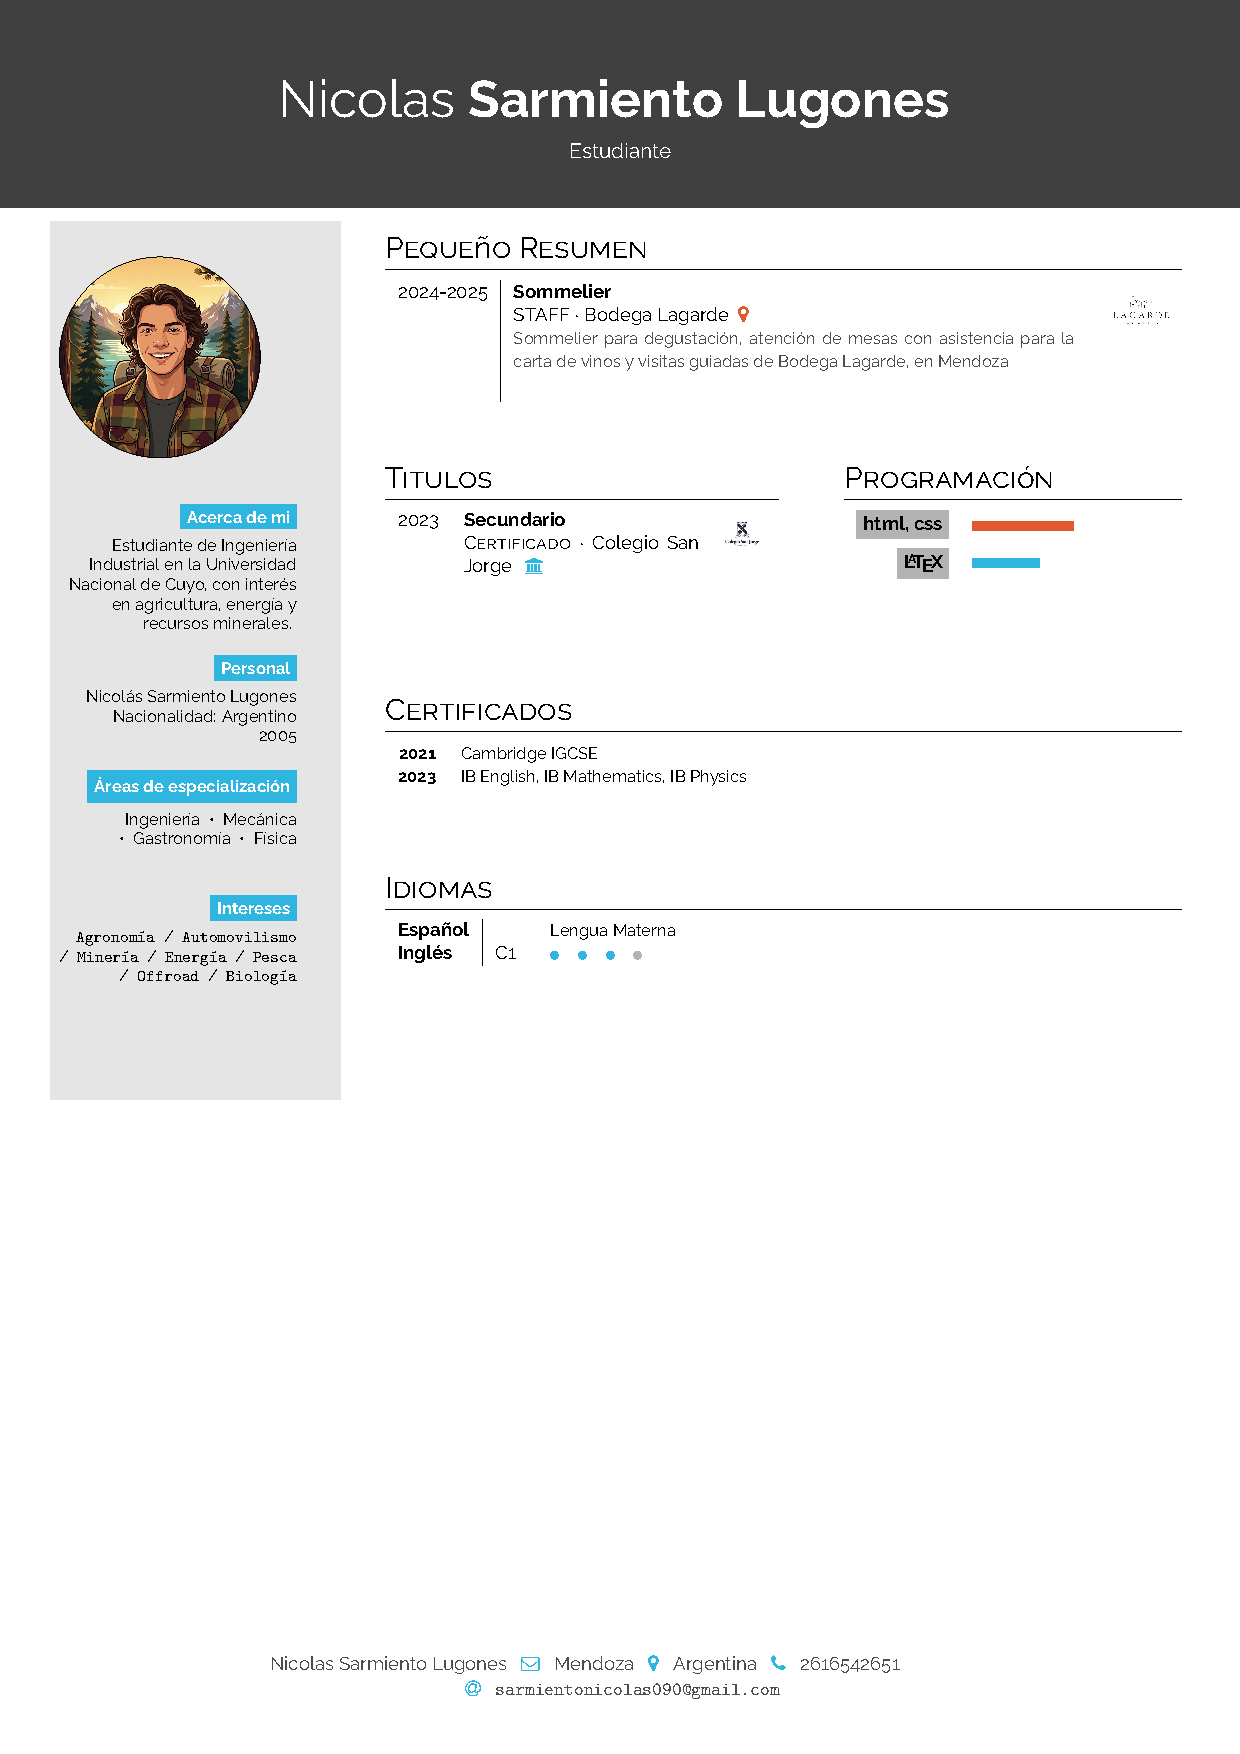
\includepdf[pages=-, pagecommand={\thispagestyle{plain}}]{cv.pdf}

% --- BIBLIOGRAFÍA ---
\bibliographystyle{splncs04}
\nocite{*}
\bibliography{Bibliografia}
\end{document}